\newcommand{\psd}[1]{{\small\sffamily{\color{blue!60}#1}}}

Same problem of linear elasticity as in tutorial 1 -- 2D bar which bends
under its own load --, is discuss here. The bar 5 m in length and 1 m in
width, and is supposed to be made up of a material with density
\(\rho=8\times 10^3\), Youngs modulus \(E=200\times 10^9\), and Poissons
ratio \(\nu=0.3\). To avoid text repetition, readers are encouraged to
go ahead with this tutorial only after tutorial 1.

As we will not use a parallel solver but a sequential one, naturally,
this tutorial leads to a slow solver than the previous tutorial 1. So
this tutorial is not for speed lovers, but rather for detailing the full
capacity of PSD. Also sequential solvers are easier to develop and
understand hence this tutorial.

As the problem remains same as tutorial 1, simply add \psd{-sequential}
flag to \psd{PSD\_PreProcess} flags from tutorial 1 for a PSD sequential
solver. The flag \psd{-sequential} signifies the use of sequential PSD
solver. So the work flow for the 2D problem would be:

\begin{lstlisting}[style=BashInputStyle]
PSD_PreProcess -problem linear_elasticity -dimension 2 -bodyforceconditions 1 \
-dirichletconditions 1 -postprocess u -sequential
\end{lstlisting}

Similar to tutorial 1, We solve the problem using the given mesh file
\psd{bar.msh}. However now we need to use \psd{PSD\_Solve\_Seq} instead
of \psd{PSD\_Solve}, as such:

\begin{lstlisting}[style=BashInputStyle]
PSD_Solve_Seq Main.edp -mesh ./../Meshes/2D/bar.msh -v 0
\end{lstlisting}

Users are encouraged to try out the 3D problem with sequential solver.
Also comparing the results from a sequential solver to that form a
parallel solver can be verified to assure that the both parallel and
sequential solvers lead to exactly the same results.

Note that for this simple problem, the bar mesh (\psd{bar.msh}) has been
provided in \psd{../Meshes/2D/"} folder, this mesh is a triangular mesh
produced with Gmsh. Moreover detailing meshing procedure is not the
propose of PSD tutorials. A user has the choice of performing their own
meshing step and providing them to PSD in
\psd{.msh}\footnote{Please use version 2} or \psd{.mesh} format, we
recommend using Salome or Gmsh meshers for creating your own geometry
and meshing them.

\subsection{Comparing CPU time}

Naturally, since we are not using parallel PSD for solving, we lose the
advantage of solving fast. To testify this claim checking solver timings
can be helpful. PSD provides means to time log your solver via
\psd{-timelog} flag. What this will do when you run your solver, on the
terminal you will have information printed on what is the amount of time
taken by each step of your solver. Warning, this will make your solver
slower, as this action involves `MPI\_Barrier' routines for correctly
timing operation.

An example work flow of 2D solver (parallel) with timelogging:

\begin{lstlisting}[style=BashInputStyle]
PSD_PreProcess -problem linear_elasticity -dimension 2 -bodyforceconditions 1 \
-dirichletconditions 1 -postprocess u -timelog
\end{lstlisting}

We solve the problem using four MPI processes, with the given mesh file
\psd{bar.msh}.

\begin{lstlisting}[style=BashInputStyle]
PSD_Solve -np 4 Main.edp -mesh ./../Meshes/2D/bar.msh -v 0
\end{lstlisting}

\begin{figure}[h!]
\centering
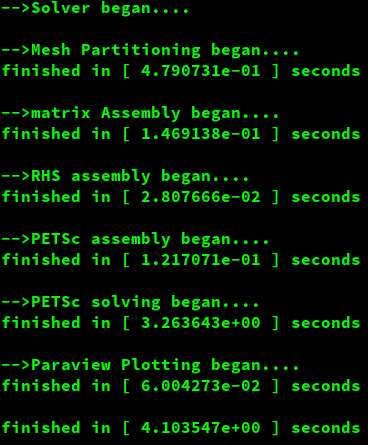
\includegraphics[width=0.4\textwidth]{./Images/le-time-par.png}
\caption{Time logging output produced for parallel run on 4 processes.\label{time-par-le}}
\end{figure}

The \cref{time-par-le} shows the time logging output produced for
parallel run on 4 processes using \psd{-timelog} flag. Take note of
timings produced for different operations of the solver.

Now let us repeat the procedure but this time use sequential solver:

\begin{lstlisting}[style=BashInputStyle]
PSD_PreProcess -problem linear_elasticity -dimension 2 -bodyforceconditions 1 \
-dirichletconditions 1 -postprocess u -timelog -sequential
\end{lstlisting}

We solve the problem now in sequential, with the given mesh file
\psd{bar.msh}.

\begin{lstlisting}[style=BashInputStyle]
PSD_Solve_Seq Main.edp -mesh ./../Meshes/2D/bar.msh -v 0
\end{lstlisting}

You should now see timings that are higher in comparison to the parallel
solver. Approximately, for large meshes using 4 MPI processes should
lead to 4 times fast solver.
